\documentclass{article}
\usepackage[utf8]{inputenc}
\textheight = 25cm 
\textwidth = 15cm
\topmargin = -3.0cm 
\oddsidemargin = 1.5cm
\usepackage{hyperref}
\hypersetup{
    colorlinks=true,
    linkcolor=blue,
    filecolor=blue,
    citecolor=black,      
    urlcolor=blue,
    }

\usepackage{float}
\usepackage{graphicx}

\usepackage{amsmath}
\usepackage{amssymb}
\usepackage{amsfonts}
\usepackage{mathtools, xparse}
\usepackage[shortlabels]{enumitem}

\usepackage[many]{tcolorbox}
\usepackage{lipsum}

\title{Tarea 3 Matemáticas Avanzadas de la Física}
\author{Cerritos Lira Carlos}
\date{16 de Abril del 2020}

\begin{document}
\maketitle

\section*{1)}
Sea $\psi(p)=\frac{d}{dp}log \Gamma(p)$ la denominada función $digamma$(ver problema $11.7$ del 
capítulo $11$). Demostrar las siguientes identidades:
\begin{enumerate}[a)]
    \item $\psi(1-p)-\psi(p)=\pi cotg(\pi p)$
    \item $\psi(p) + \psi(p + 1/2) + 2log2 = 2\psi(2p)$
    \item Usar las propiedades de la función digamma para Demostrar que:
    \[ \psi(n+1/2) = -\gamma - 2log2 + 2\sum_{k=1}^n \frac{1}{2k-1}, \quad n=1,2...\]
    donde $\gamma = -\psi(1) = -\Gamma'(1) = 0.05721566...$ es la constante de Euler.
\end{enumerate} 
\begin{tcolorbox}[breakable]
    \subsubsection*{a)}
    Comenzamos con la formula de reflección de Euler:
    \begin{align*}
        \Gamma(p)\Gamma(1-p) &= \frac{\pi}{sin\pi p} \\
        log(\Gamma(p)) + log(\Gamma(1-p)) &= log\pi - log(sin\pi p) \\
        \frac{\Gamma'(p)}{\Gamma(p)}-\frac{\Gamma'(1-p)}{\Gamma(1-p)} &= -\frac{\pi cos\pi p}{sin\pi p} \\
        \psi(p) - \psi(1-p) &= -\pi cot\pi p \\
        \psi(1-p) - \psi(p) &= \pi cot\pi p 
    \end{align*}

    \subsubsection*{b)}
    Comenzamos con la formula de duplicación de Legendre:
    \begin{align*}
        \Gamma(p)\Gamma(p+1/2) &= 2^{1-2p}\sqrt{\pi}\Gamma(2p)\\
        log(\Gamma(p))+log(\Gamma(p+1/2)) &= log(2)(1-2p) +log(\Gamma(2p)) \\
        \frac{\Gamma'(p)}{\Gamma(p)} + \frac{\Gamma'(p+1/2)}{\Gamma(p+1/2)} &= -2log2 + 2\frac{\Gamma'(2p)}{\Gamma(2p)} \\
        \psi(p) + \psi(p + 1/2) + 2log2 &= 2\psi(2p)
    \end{align*}

    \subsubsection*{c)}
    Despejamos $\psi(n+1/2)$ de la última expresión:
    \begin{align*}
        \psi(n+1/2) 
        &= - 2log2 + 2\psi(2n)-\psi(n) \\
        &= -2log2 
        + 2\left(\sum_{k=1}^{2n-1} \frac{1}{k} - \gamma \right) -\left( \sum_{k=1}^{n-1} \frac{1}{k} - \gamma \right) \\
        &= -\gamma -2log2 + 2\sum_{k=1}^{n} \frac{1}{2k-1}
    \end{align*}

\end{tcolorbox}

\section*{2)}
Sea $F(x) = e^{-x^2}\int_{0}^{x}e^{t^2}dt$. Demostrar que $F$ verifica la ecuación diferencial 
$F'(x) + 2xF(x) = 1$. Usar este hecho para demostrar la expansión:
\[ F(x) = \sum_{n=0}^\infty \frac{(-1)^n2^nx^{2n+1}}{(2n+1)!!}, \quad  \Big|x \Big| < \infty \]
Por último demostrar que $F(x) \sim \frac{1}{2x}$ a medida que $x \to \infty$ y hacer un esbozo
de la gráfica de $F$. Esta función está relacionada con la función error y aparece en la teoría de 
propagación de ondas electromagnéticas sobre la superfiece de la Tierra.
\begin{tcolorbox}[breakable]
    \subsubsection*{Primer relación}
    Hacemos las cuentas para obtener $F'(x) + 2xF(x)$:
    \begin{align*}
        F'(x) + 2xF(x) 
        &= -2xe^{-x^2}\int_0^x e^{t^2}dt + e^{-x^2}e^{x^2} + 2F(x) \\
        &= -2xe^{-x^2}\int_0^x e^{t^2}dt + 1 + 2F(x) \\
        &= -2xe^{-x^2}\int_0^x e^{t^2}dt + 1 + 2xe^{-x^2}\int_{0}^x e^{t^2} dt = 1 
    \end{align*}
    \subsubsection*{Expansión}
    queremos que la función sea de la forma:
    \begin{align*}
        F(x) &= \sum_{n=0}^\infty a_n x^n, 
        \quad F'(x) = \sum_{n=1}^\infty na_n x^{n-1},
        \quad F''(x) = \sum_{n=2}^\infty n(n-1)a_n x^{n-2}
    \end{align*}
    se debe satisfacer la ecuación diferencial:
    \begin{align*}
        F''(x) + 2xF'(x) + 2F(x) 
        &= \sum_{n=2}^\infty n(n-1)a_n x^{n-2} + 2x\sum_{n=1}^\infty na_n x^{n-1} + 2\sum_{n=0}^\infty a_n x^n\\
        &= \sum_{n=0}^\infty (n+1)(n+1)a_{n+2}x^n + \sum_{n=1}^\infty 2na_nx^n + \sum_{n=0}^\infty 2a_nx^n \\
        &= 2a_{2} + a_0 + \sum_{n=1}^\infty ((n+2)(n+1)a_{n+2}+2(n+1)a_n) x^n \\
        &= 0
    \end{align*}
    se tienen las condiciones:
    \begin{align*}
        2a_2 + a_0 &= 0 \\
        (n+2)(n+1)a_{n+2}+2(n+1)a_n &= 0
    \end{align*}
    de donde obtenemos la relación:
    \begin{align*}
        a_{n+2} 
        &= -\frac{2(n+1)}{(n+2)(n+1)}a_n \\
        &= -\frac{2}{n+2}a_n
    \end{align*}
    usando la condición $F(0) = 0, F'(0) = 1$ obtenemos $a_0 = 0, a_1 = 1$, por lo tanto se tiene:
    \begin{align*}
        a_{2n} &= 0 \\
        a_{2n+1} &= \frac{(-1)^{n}2^{n}}{(2n+1)!!}
    \end{align*}
    substituyendo obtenemos la expansión deseada:
    \begin{align*}
        F(x) = \sum_{n=0}^\infty \frac{(-1)^n2^nx^{2n+1}}{(2n+1)!!}
    \end{align*}
    \subsubsection*{Relación $F(x)\sim \frac{1}{2x}$}
    Queremos saber si se cumple:
    \[ \lim_{x\to \infty} F(x)2x = 1 \]
    primero calcularemos $\lim_{x \to \infty} \frac{\int_0^x e^{t^2}dt}{e^{x^2}}$:
    \begin{align*}
        \lim_{x \to \infty} \frac{\int_0^x e^{t^2}dt}{e^{x^2}}
        &= \lim_{x \to \infty} \frac{e^{x^2}}{2xe^{x^2}} \\
        &= \lim_{x \to \infty} \frac{1}{2x} \\
        &= 0
    \end{align*}
    usando esta información podemos calcular $\lim_{x \to \infty} F'(x)$:
    \begin{align*}
        \lim_{x \to \infty} F'(x) 
        &= \lim_{x \to \infty}\left(-2xe^{-x^2}\int_{0}^x e^{t^2}dt + 1\right) \\
        &= \lim_{x \to \infty}\left(\frac{-2x\int_0^x e^{t^2}dt }{e^{x^2}} \right) + 1 \\
        &= \lim_{x \to \infty}\left(\frac{-2\int_0^x e^{t^2}dt + -2x^2e^{x^2}}{e^{x^2}} \right) + 1 \\
        &= \lim_{x \to \infty}\left(\frac{1}{x}\frac{\int_0^x e^{t^2}dt}{e^{x^2}} \right) - 1 + 1 \\
        &= \lim_{x \to \infty}\left( \frac{1}{x} \right) \lim_{x \to \infty} \left(\frac{\int_0^xe^{t^2}dt}{e^{x^2}} \right) \\
        &= 0
    \end{align*}
    ahora bien tomando limite de ambos lados para la primer relación tenemos:
    \begin{align*}
        \lim_{x \to \infty}(F'(x) + 2xF(x)) &= \lim_{x \to \infty} 1 \\
        \lim_{x \to \infty}F'(x) + \lim_{x \to \infty} 2xF(x) &= 1 \\
        \lim_{x \to \infty} 2xF(x) &= 1
    \end{align*}
    que es lo que se quería demostrar. 

    \subsubsection*{Gráfica de la función}
    \begin{figure}[H]
        \centering
        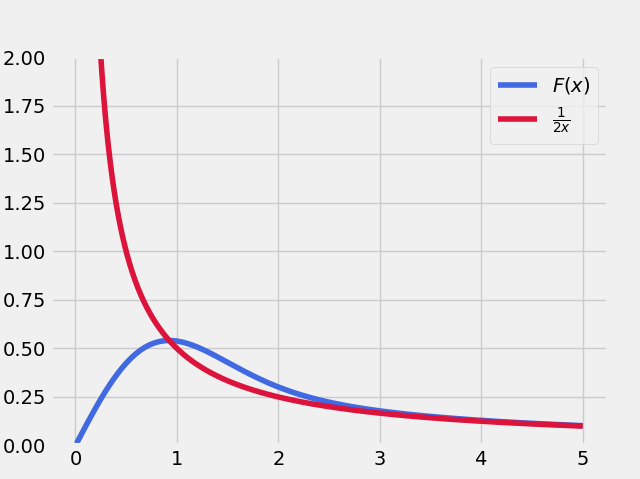
\includegraphics[scale=0.6]{images/p2_grafica.png}
    \end{figure}
\end{tcolorbox}

\section*{3)}
Obtener las series asintóticas de las sigueintes integrales y comprobar la identidad $(10.7)$ ó $(1.7)$
del Capítulo $11$ del Boas:
\begin{enumerate}[a)]
    \item $G(\epsilon) = \int_0^\infty \frac{e^{-x}}{1+\epsilon x}dx = \sum_{n=0}^\infty (-1)^n n! \epsilon^n, \quad \epsilon \to 0^+$
    \item $I(\epsilon) = \int_{-\infty}^\infty e^{-x^2/2-\epsilon x^4}dx = \sqrt{2\pi} \left( 1 + \sum_{n=1}^\infty \frac{(-1)^n (4n-1)!!}{n!}\epsilon^n \right), \quad \epsilon \to 0^+$
    \item $Ei(x) = \int_{-\infty}^x \frac{e^t}{t}dt = \frac{e^x}{x}\sum_{n=0}^\infty \frac{n!}{x^n}, \quad x \to \infty$
\end{enumerate}
\begin{tcolorbox}[breakable]
    \subsubsection*{a)}
    Integramos por partes para obtener los términos $\epsilon^n$ de la serie:
    \begin{align*}
        G(\epsilon) 
        &= \int_{0}^\infty \frac{e^{-x}}{1+\epsilon x}dx \\
        &= 1-\epsilon \int_0^\infty \frac{e^{-x}}{(1+\epsilon x)^2}dx \\
        &= 1-\epsilon + ... + (-1)^N N! \epsilon^N + (-1)^{N+1} (N+1)! \epsilon^{N+1} \int_{0}^\infty \frac{e^{-x}}{(1+\epsilon x)^{N+1}}dx
    \end{align*}
    veremos que la serie $\sum_{n=0}^\infty (-1)^n n! \epsilon^n = \sum_{n=0}^\infty a_n \epsilon^n$ es asintótica:
    \begin{align*}
        L 
        &= \lim_{\epsilon \to 0^+}\frac{|G(\epsilon) - \sum_{n=0}^Na_n \epsilon^n |}{\epsilon^N} \\
        &= \lim_{\epsilon \to 0^+}\frac{|(-1)^{N+1} (N+1)! \epsilon^{N+1} \int_{0}^\infty \frac{e^{-x}}{(1+\epsilon x)^{N+1}}dx|}{\epsilon^N} \\
        &= \lim_{\epsilon \to 0^+} (N+1)! \epsilon |\int_{0}^\infty \frac{e^{-x}}{(1+\epsilon x)^N}dx| \\
        &\leq \lim_{\epsilon \to 0^+} (N+1)! \epsilon \int_{0}^\infty e^{-x}dx \\
        &= \lim_{\epsilon \to 0^+} (N+1)! \epsilon \\
        &= 0
    \end{align*}
    haciendo sandwich podemos ver que $L=0$, por lo tanto la serie es asintótica por definición.

    \subsubsection*{b)}
    Hacemos serie de Tylor para obtener los términos $\epsilon^n$ de la serie:
    \begin{align*}
        e^{-x^2/2-\epsilon x^4} 
        &= e^{-x^2/2}\left( \sum_{n=0}^N \frac{(-1)^n}{n!} \epsilon^n x^{4n} + \epsilon^{N+1}r_{N+1}(x) \right) \\ 
        &= \sum_{n=0}^N \frac{(-1)^n}{n!} e^{-x^2/2} x^{4n} \epsilon^n  + \epsilon^{N+1} e^{-x^2/2} r_{N+1}(x) 
    \end{align*}
    por el teorema de Tylor sabemos que se cumple:
    \begin{align*}
        |r_{N+1}(x)| 
        &= \Big|(-1)^{N+1}\frac{e^c}{(N+1)!}x^{4(N+1)} \Big| \quad c \in (-\epsilon x^4,0) \\
        &\leq x^{4(N+1)}
    \end{align*}
    integrando término por término obtenemos:
    \begin{align*}
        I(\epsilon)
        &= \int_{-\infty}^\infty e^{-x^2/2-\epsilon x^4} \\
        &= \int_{-\infty}^\infty \left( \sum_{n=0}^N \frac{(-1)^n}{n!} e^{-x^2/2} x^{4n} \epsilon^n  + \epsilon^{N+1} e^{-x^2/2} r_{N+1}(x) \right)dx \\
        &= \sum_{n=0}^N \left( \frac{(-1)^n}{n!} \int_{-\infty}^\infty e^{-x^2/2}x^{4n}dx \epsilon^n \right)  + \epsilon^{N+1}\int_{-\infty}^\infty e^{-x^2/2}r_{N+1(x)} dx \\
        &= \sqrt{2\pi} \sum_{n=0}^N a_n \epsilon^n + \epsilon^{N+1}\int_{-\infty}^\infty e^{-x^2/2}r_{N+1}(x) dx 
    \end{align*}
    donde $a_n = \frac{1}{\sqrt{2\pi}} \int_{-\infty}^\infty e^{-x^2/2}x^{4n}dx = \frac{(-1)^n(4n-1)!!}{n!}$.
    veremos que se satisface la condición $1.7$:
    \begin{align*}
        L 
        &= \lim_{\epsilon \to 0^+} \frac{|I(\epsilon) - \sum_{n=0}^N a_n\epsilon^n|}{\epsilon^N} \\
        &= \lim_{\epsilon \to 0^+} \frac{|\epsilon^{N+1} \int_{-\infty}^\infty e^{-x^2/2}r_{N+1}(x)dx |}{\epsilon^N} \\
        &\leq \lim_{\epsilon \to 0^+} \epsilon \int_{-\infty}^\infty x^{4(N+1)}e^{-x^2/2}dx \\
        &= \lim_{\epsilon \to 0^+} \epsilon \sqrt{2\pi} a_{n+1} \\
        &= 0
    \end{align*}
    haciendo sandwich nuevamente podemos ver que $L=0$, por lo tanto la serie es asintótica por definición.
    \subsubsection*{c)}
    Integramos por partes para obtener los terminos $\frac{1}{x}$ de la serie:
    \begin{align*}
        \int_{-\infty}^x \frac{e^t}{t}dt 
        &= \frac{e^t}{t} \Big|_{-\infty}^x + \int_{-\infty}^x \frac{e^t}{t^2}dt \\
        &= \frac{e^x}{x} + \frac{e^t}{t^2} \Big|_{-\infty}^x + \int_{-\infty}^x 2 \frac{e^t}{t^3}dt \\
        &= \frac{e^x}{x} \left(1 + \frac{1}{x} + \frac{2}{x^2} \right) + (3)(2) \int_{-\infty}^x \frac{e^t}{t^4} dt \\
        &= \frac{e^x}{x} \sum_{n=0}^N \frac{n!}{x^n} + (N+1)!\int_{-\infty}^x \frac{e^t}{t^{N+2}}dt 
    \end{align*}
    veremos que se satisface la condicion más general:
    \begin{align*}
        I 
        &=\lim_{x\to \infty} \frac{|Ei(x) - \sum_{n=0}^N \phi_n(x)|}{\phi_N(x)} \\
        &=\lim_{x\to \infty} \frac{(N+1)! \int_{-\infty}^x \frac{e^t}{t^{N+2}}}{\frac{e^x}{x}\frac{N!}{x^N}} \\
        &=\lim_{x\to \infty} \frac{(N+1)x^{N+1}\int_{-\infty}^x \frac{e^t}{t^{N+2}}}{e^x} \\
        &= 0
    \end{align*}
\end{tcolorbox}
\end{document}